
\section{Aufgabe 2 - Reaktionsspiel}
\label{sec:aufgabe-2---reaktionsspiel}

Es soll eine Schaltung implementiert werden, welche ein lichtbasiertes Reaktionsspiel darstellt.
Die Schaltung soll aus fünf LEDs bestehen, welche der Reihe nach leuchten und erlöschen.
D.h., LED 1 leuchtet, LED 1 erlischt und LED 2 leuchtet, LED 2 erlischt und LED 3 leuchtet, u.s.w..
Sobald die letzte LED erlischt soll die erste LED wieder leuchten und der Rythmus von neuen beginnen.

Die LEDs werden in der Reihenfolge Rot - Gelb - Grün - Gelb - Rot geschaltet und angeordnet.
Des weiteren wird ein Taster eingebaut.
Wird der Taster gedrückt, wenn die grüne LED leuchtet, halbiert sich die Zeit zwischen der die LEDs geschaltet werden.
D.h., bleibt eine LED fünf Sekunden eingeschaltet, bevor die nächste LED geschaltet wird, so bleibt sie danach nur 2,5 Sekunden lang eingeschaltet.
Wird der Taster erneut gedrückt, wenn die grüne LED leichtet, halbiert sich die Zeit erneut auf 1,25 Sekunden, u.s.w..

Wird der Taster gedrückt, wenn die grüne LED nicht leuchtet, wird die Zeit wieder auf den ursprünglichen Wert gesetzt.
In diesem Beispiel also zurück auf fünf Sekunden.
In diesem Fall sollen auch alle LEDs gleichzeitig drei mal blinken, bevor das Spiel schlussendlich von vorne beginnt.

\subsection{Materialien}
\label{subsec:a2-materialien}

\begin{table}[h]
    \centering
    \caption{Aufgabe 2 - Verwendete Materialien}
    \label{tab:a2-materialien}
    \begin{tabular}{| l | l | l |}
        \hline
        Bezeichnung & Eigenschaften & Menge \\
        \hline
        Widerstand  & $150\Omega$   & 5     \\
        & Braun - Grün - Braun - Gold & \\
        Widerstand & $10k\Omega$ & 1 \\
        & Braun - Schwarz - Orange - Gold & \\
        LED & Rot & 2 \\
        LED & Gelb & 2 \\
        LED & Grün & 1 \\
        Taster & 4 Polig & 1 \\
        Mikrocontroller & Arduino Uno R3 & 1 \\
        \hline
    \end{tabular}
\end{table}

\subsection{Vorbereitung}
\label{subsec:a2-vorbereitung}

Für den ersten Teil muss wieder der Vorwiderstand der LEDs berechnet werden.
Die Berechnung und des Widerstands und die reale Auswahl aus der E6-Reihe erfolgt wie in Sektion \ref{subsec:A1-vorbereitung}.
D.h., es wurden $200\Omega$ berechnet und der $150\Omega$ Widerstand aus der E6-Reihe ausgewählt.

Der zweite Teil bestand aus zwei Fragestellungen.
Erstens, wie kann ein Mikrocontroller-Programm unterbrochen werden, um ,z.B., einen Druck auf einen Taster zu erkennen.
Dies kann mithilfe eines sogenannten \textit{Interrupts} implementiert werden.
Dafür wird ein Pin als Input-PullUp-Pin angelegt und für diesen Pin eine Funktion definiert, welche aufgerufen wird, sobald der Taster gedrückt wird.

Zweitens, wie kann ermittelt werden, ob der Taster zum richtigen oder falschen Zeitpunkt gedrückt wurde.
Dafür kann eine Variable mit dem \textit{volatile}-Schlüsselwort angelegt werden.
Damit wird die Variable nicht in einem Zwischenspeicher behalten, sondern wird immer vom Hauptspeicher gelesen, wenn sie verwendet wird.
Diese Variable kann die Werte "wahr", bzw.\ "true", und "falsch", bzw "false", annehmen.
Wird der Button gedrückt kann die Variable auf "wahr" gesetzt werden, ansonsten auf "falsch".
In der Programmlogik selbst kann dann überprüft werden, welchen Wert die Variable momentan besitzt.
Damit kann ausgewertet werden, ob sie zum "richtigen" Zeitpunkt den Wert "wahr" hat, oder nicht.

\subsection{Praktikumsaufgabe}
\label{subsec:a2-praktikumsaufgabe2}

In Abbildung \ref{fig:implementierter-stromkreis-a2} ist die implementierte Schaltung zu sehen.
Zur Klärung sei gesagt, dass das blaue Kabel nur mit Spalte 15 verbunden ist und nicht mit einem der Widerstände, obwohl das Bild es vermuten lässt.

\begin{figure}[ht]
    \centering
    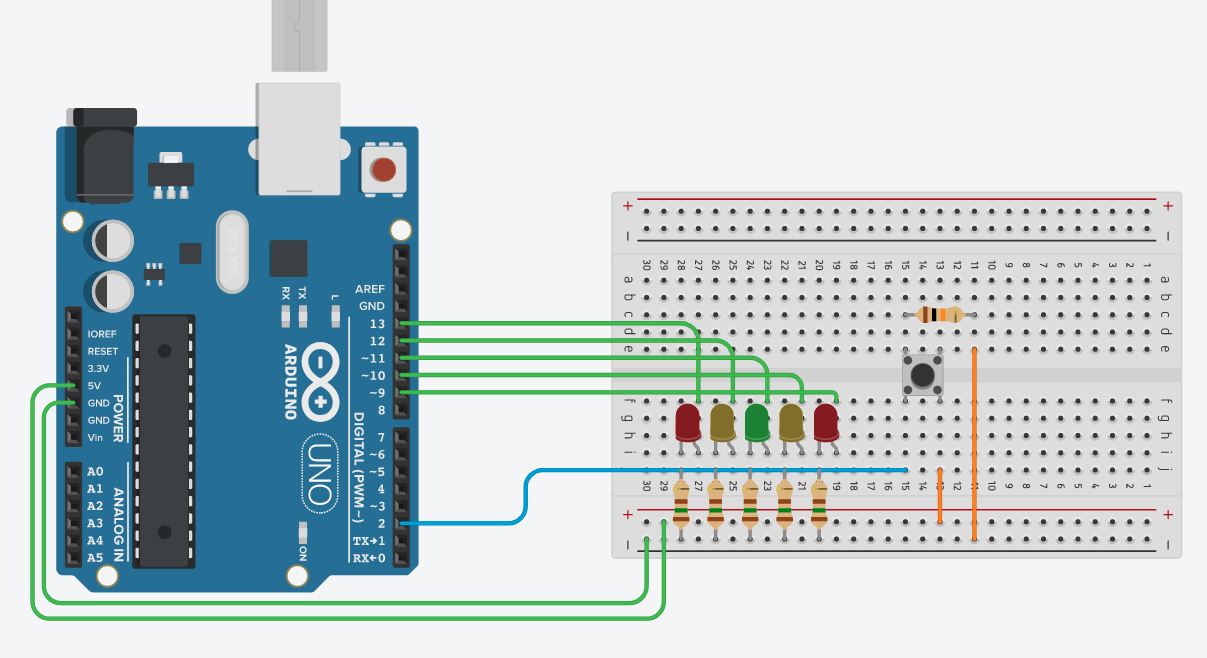
\includegraphics[width=\textwidth]{pictures/a2-praktik.png}
    \caption{Implementierter Stromkreis von Aufgabe 2}
    \label{fig:implementierter-stromkreis-a2}
\end{figure}

Weiters ist die Wahl der Pins zu erkennen.
Die Wahl viel auf die Pins 9 bis 13 zur Steuerung der LEDs und auf Pin 2 zur Erkennung des Tastendrucks.
Die Pins zur Ansteuerung der LEDs wurde willkürlich getroffen.
Es handelt sich nur von oben nach unten um die ersten, zur Verfügung stehenden Pins.
Pin 2 wurde gewählt, da nur Pin 2 und 3 in der Lage sind, an einen Interrupt gekoppelt zu werden.

\newpage

Im Schaltkreis ist weiters der Taster zu sehen, der mit einem Pull-Up-Widerstand, wie in Sektion \ref{subsec:pullup} zu sehen, versehen ist.
Die Terminals an der Spalte 15 auf beiden Seiten sind verbunden, die Terminal an den Spalten 15 und 13 werden bei einem Tastendruck verbunden.
Damit ergibt sich das Teilschaltbild des Tasters, dass in Abbildung \ref{fig:schaltung-taster-pull-up} zu sehen ist.
Die alleinstehenden Zahlen geben die zugehörige Spalte des Steckbrettes an.
Des weiteren sei gesagt, dass in der Abbildung zwei Schalter zu sehen sind, diese repräsentieren die zwei vorhanden Terminals des echten Schalters.
Bei Tastendruck werden beide gleichzeitig geschlossen.

\begin{figure}[h]
    \centering
    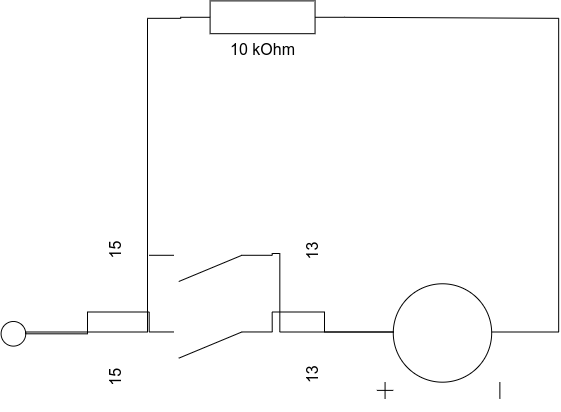
\includegraphics[width=0.58\textwidth]{pictures/a2-taster.png}
    \caption{Schaltung des Tasters mit Pull-Up Widerstand}
    \label{fig:schaltung-taster-pull-up}
\end{figure}

Im nachfolgendem Text wird der Programmcode der Aufgabe erläutert.
Einzelne Teile des Codes werden ausgewählt und beschrieben.
Am Ende dieser Sektion befindet sich der vollständige Programmcode.

\begin{lstlisting}[language=C,label={lst:a2-const-pin}, caption={Setzen der Pin-Konstanten}]
onst int NUM_PINS = 5;
const int WINNING_PIN_INDEX = 2;
const int PINS[] = {
	13, 12, 11, 10, 9
};
const int PIN_BUTTON = 2;
\end{lstlisting}

In Listing \ref{lst:a2-const-pin} werden die Nummern der Pins angelegt.
Die Besonderheit gegenüber der vorherigen Sektion, Sektion \ref{sec:aufgabe-1}, ist die Verwendung eines Arrays.
In diesem werden die verwendeten Pinnummern zu Ansteuerung der LEDs angegeben.
Mit $NUM\_PINS$ wird die Länge des Arrays angegeben.
Solch eine Angabe ist nützlich, da die Länge eines Arrays in der gegebenen Programmiersprache, C, nicht trivial findbar ist.

Um in C die Länge eines Arrays zu bestimmen, müsste zuerst mittels $sizeof(PINS)$ die Menge an Speicher ermittelt werden, die das Arrays belegt.
Dieser Wert müsste sodann durch das Ergebnis von $sizeof(int)$, die Menge an Speicher die ein Integer-Wert im Speicher belegt, dividiert werden.
Das Ergebnis aus $sizeof(PINS) / sizeof(int)$ würde dann die Länge des Arrays ergeben.
Einfacher ist es daher, die Größe als Konstante anzugeben, wenn diese, wie in diesem Fall, bekannt ist.
Mit der Konstante $PIN\_BUTTON$ wird die Pinnummer des Pins angegeben, welcher später den Zustand des Tasters erkennt.

Die Konstante $WINNING\_PIN\_INDEX$ gibt an, welcher Index des Pin-Arrays die grüne LED darstellt,
D.h., die der Taster gedrückt, wenn der Pin von $PINS[WINNING\_PIN\_INDEX]$ eingeschaltet ist, ist zum richtigen Zeitpunkt gedrückt worden.

\begin{lstlisting}[language=C,label={lst:a2-const-interval}, caption={Standard Interval zum LED wechsel}]
const unsigned long INTERVAL_DEFAULT = 5000;
\end{lstlisting}

\newpage

Mit der Konstanten die in Listing \ref{lst:a2-const-pin} angegeben ist, wird das Standardinterval angegeben, mit dem bei den LEDs weitergesprungen wird.
D.h., nach Ablauf der Zeit von $INTERVAL\_DEFAULT$, in Millisekunden, wird zur nächsten LED gesprungen, wenn das Spiel neu gestartet wurde.


\begin{lstlisting}[language=C,label={lst:a2-zeitmessung-variablen}, caption={Variablen zur Zeitmessung}]
unsigned long current_millis = 0;
unsigned long previous_millis = 0;
unsigned long interval = INTERVAL_DEFAULT;
\end{lstlisting}

Die Variablen in Listing \ref{lst:a2-zeitmessung-variablen} werden dazu verwendet, die vergangene Zeit im Programm mitzuverfolgen.
In $current\_millis$ wird gespeichert, wie viel Zeit seit dem Programmstart vergangen ist.
Der Wert in $previous\_millis$ gibt an, zu welchem Zeitpunkt die letzte Aktion durchgeführt wird.
Die Bedeutung dieser Variable wird im Verlauf des Programmcodes klarer.
In $interval$ ist das derzeitige Interval zwischen Wechseln der LEDs gespeichert.
Zu Beginn wird sie mit der Konstante aus Listing \ref{lst:a2-const-interval} initialisiert.
Sie wird bei jedem Neustart des Spiels auf diesen Wert zurückgesetzt.

\begin{lstlisting}[language=C,label={lst:a2-game-state-variablen}, caption={Variablen zur Zustandsbestimmung des Spiels}]
int pin_index = 0;

volatile bool button_pressed = false;
volatile bool game_over = false;
\end{lstlisting}

Durch die Variablen in Listing \ref{lst:a2-game-state-variablen} wird der derzeitige Zustand des Spiels mitverfolgt.
Sie haben zusätzlich zum Typ noch das Schlüsselwort $volatile$, welches im zweiten Teil der Sektion \ref{subsec:a2-vorbereitung} beschrieben wurde.
Diese Schlüsselwort benötigen sie, da die Variablen in einem Interrupt verändert werden und dadurch direkt vom Speicher ausgelesen werden müssen.
Eine Annäherung des mit diesen Variablen bewirkten Zustandsverlauf kann in Abbildung \ref{fig:annäherung-des-spielverlaufs} abgelesen werden.

\begin{figure}[ht]
    \centering
    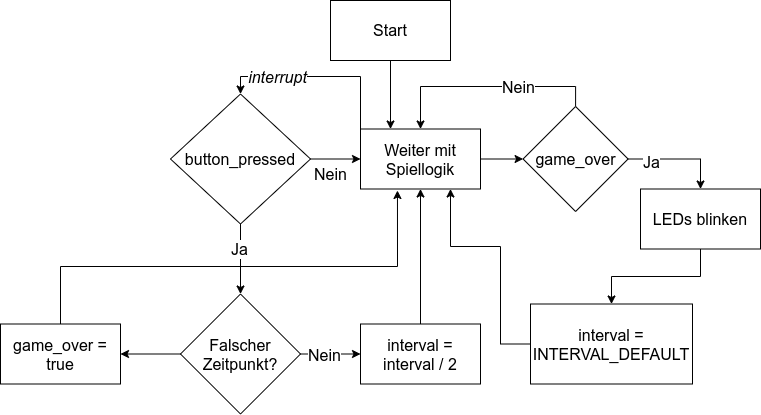
\includegraphics[width=\textwidth]{pictures/a2-game-state.png}
    \caption{Annäherung des Spielverlaufs}
    \label{fig:annäherung-des-spielverlaufs}
\end{figure}


Die Variable $pin\_index$ ist nicht mittels $volatile$ markiert, da sie sich nur in der Hauptschleife des Programms ändert.
Nach Ablauf von $interval$ wird sie um 1 erhöht bis zu einem Maximum von $NUM\_PINS - 1$.
Würde sie den Wert $NUM\_PINS$ annehmen, wird sie wieder auf 0 zurückgesetzt.
Diese Variable gibt an, welcher Index, von 0 beginnend, aus $PINS$ verwendet wird, um eine LED anzusteuern.
D.h., $pin\_index = 0 \Rightarrow Pin13 = HIGH$, $pin\_index = 1 \Rightarrow Pin12 = HIGH$, u.s.w..

\newpage

\begin{lstlisting}[language=C,label={lst:a2-serial-begin}, caption={Einstellen der seriellen Schnittstelle}]
void setup() {
  Serial.begin(9600);
\end{lstlisting}

Mit dem Kommando in Listing \ref{lst:a2-serial-begin} wird eine serielle Verbindung zu einem verbundenem Computer hergestellt.
Damit kann später im Programm Text an den Computer übertragen oder vom Computer auf den Mikrocontroller gesendet werden.
Das Argument der Methode, $9600$ gibt die Baudrate an.

\begin{lstlisting}[language=C,label={lst:a2-pin-setup}, caption={Konfiguration der Pins}]
int i;
for (i = 0; i < NUM_PINS; i++) {
    pinMode(PINS[i], OUTPUT);
}
\end{lstlisting}

In Listing \ref{lst:a2-pin-setup} werden die Pins durchgegangen.
Hier wird das in Listing \ref{lst:a2-const-pin} angelegte Array zum ersten Mal verwendet.
Es werden hier alle Pinnummern in dem Arrays durchgelaufen und als Output eingestellt.
Dadurch muss nicht jede Pinnummer einzeln eingerichtet werden.

\newpage

\begin{lstlisting}[language=C,label={lst:a2-button setup}, caption={Einstellen des Buttons}]
pinMode(PIN_BUTTON, INPUT_PULLUP);

attachInterrupt(
    digitalPinToInterrupt(PIN_BUTTON),
    on_button_change,
    CHANGE);
\end{lstlisting}

Der Code in Listing \ref{lst:a2-button setup} setzt nun den Pin, der an dem Taster angeschlossen ist, auf Input-PullUp und verknüpft ihn mit einem Interrupt.
Die Funktion $on\_button\_change$ wird nun aufgerufen, jedes mal wenn der Taster manipuliert wird.
Der Parameter dritte Parameter der $attachInterrupt$-Methode, in diesem Fall $CHANGE$, gibt an was passieren muss damit die Methode aufgerufen wird.
$CHANGE$ beduetet, dass jedes mal wenn sich das Potenzial ändert, daher entweder von $5V$ auf $0V$ fällt oder von $0V$ auf $5V$ steigt, der Interrupt ausgeführt wird.

Des weiteren gibt es noch weitere Werte, die übergeben werden können, welche verschieden Zustände abbilden.

\begin{itemize}
    \item $LOW$, der Interrupt wird ausgeführt, wenn am Pin $0V$ anliegen
    \item $CHANGE$, der Interrupt wird ausgeführt, wenn sich das Potenzial am Pin ändert
    \item $RISING$, der Interrupt wird ausgeführt, wenn die Spannung am Pin von $0V$ auf $5V$ steigt
    \item $FALLING$, der Interrupt wird ausgeführt, wenn die Spannung am Pin von $5V$ auf $0V$ fällt
\end{itemize}

\begin{lstlisting}[language=C,label={lst:a2-init}, caption={Setzen der Standardwerte}]
  init_game();
}

void init_game() {
  game_over = false;
  interval = INTERVAL_DEFAULT;
  pin_index = 0;
  digitalWrite(PINS[0], HIGH);
}
\end{lstlisting}

Listing \ref{lst:a2-init} zeigt die Methode, die aufgerufen wird, wenn das Spiel neu gestartet wird.
Der Aufruf von $init\_game()$ zu Begin des Listings ist noch in der $setup()$-Methode zu finden.
Dadurch werden noch vor Spielbeginn die Werte richtig gesetzt.

In der $init\_game()$-Methode wird des Zustand mittels $game\_over$ zurückgesetzt.
Das Intervall zwischen den LED wechseln wird auf den Standardwert gesetzt.
Die aktive LED wird mittels $pin\_index = 0$ auf die Erste gesetzt und mit dem Aufruf von $digitalWrite(\dots)$ eingeschaltet.

\begin{lstlisting}[language=C,label={lst:a2-button-interrupt}, caption={Interrupt Methoden des Tasters}]
void on_button_change() {
  int button_state = digitalRead(PIN_BUTTON);
  if (button_state == HIGH) {
   	on_button_rising();
  } else {
    on_button_falling();
  }
}

void on_button_rising() {
  button_pressed = true;

  if (pin_index == WINNING_PIN_INDEX &&
     !game_over) {
    interval = interval / 2;
  } else {
    game_over = true;
  }
}

void on_button_falling() {
  button_pressed = false;
}
\end{lstlisting}

Obwohl die Methoden, welche die Logik des Interrupts darstellen, am Ende des Codes liegen, werden sie hier besprochen.
Damit kann ein Kontext für andere Codeteile erzeugt werden.

\newpage

In Listing \ref{lst:a2-button-interrupt} wird die in Listing \ref{lst:a2-button setup} verwendete Methode gezeigt.
Zu Beginn von $on\_button\_change()$ wird der Zustand des Tasters ausgelesen.
Liegen zum Zeitpunkt des Aufrufs $5V$ am Pin an, so wird $on\_button\_rising()$ aufgerufen, ansonsten wird $on\_button\_falling()$ verwendetet.
Dieser Distinktion muss verwendet werden, da nur ein Interrupt pro Pin angelegt werden kann.
Es können die entsprechenden Methoden nicht gleichzeitig direkt an den Pin angehängt werden.
Daher muss die Methode $on\_button\_change()$ diese Unterscheidung durchführen.

In $on\_button\_rising()$ wird zuerst der Zustand von $button\_pressed$ auf $true$ gesetzt.
Damit kann in der Programmschleife erkannt werden, ob der Taster gedrückt wird oder nicht.
Danach wird überprüft welche LED zurzeit leuchtet, indem der Wert in $pin\_index$ überprüft wird und ob das Spiel bereits vorbei ist.
Die letztere Überprüfung wird gemacht, da der Taster auch dann getätigt werden kann, wenn, z.b., alle LEDs blinken.
Wurde der Taster nicht zum richtigen Zeitpunkt getätigt, so wird der Zustand des Spiels auf "Game Over" gesetzt, indem die enstprechende Variable auf $true$ gesetzt wird.

\begin{lstlisting}[language=C,label={lst:a2-hilfsmethoden}, caption={Hilfsmethoden}]
void blink_all() {
  int j;
  for (j = 0; j < 3; j++) {
    int i;
    write_to_all(HIGH);
    delay(500);
    write_to_all(LOW);
    delay(500);
  }
}

void write_to_all(int state) {
  int i;
  for (i = 0; i < NUM_PINS; i++) {
    digitalWrite(PINS[i], state);
  }
}

void increase_pin_index() {
    pin_index++;
    if (pin_index >= NUM_PINS){
      pin_index = 0;
    }
}
\end{lstlisting}

\newpage

In Listing \ref{lst:a2-hilfsmethoden} werden die verwendeten Hilfsmethoden gezeigt.
Für $write\_to\_all$ kann der gewünschte Zustand übergeben werden, $HIGH$ oder $LOW$, und dieser wird, ähnlich wie in $setup()$, mittels einer Schleife an alle Pins im $PINS$-Array übernommen.
$blink\_all$ wird verwendet, um das Blinken der LEDs am Ende des Spiels zu implementieren.
Es werden hier drei mal alle Pins im $PINS$-Array erst mittels $write\_to\_all(HIGH)$ eingeschaltet.
Danach wird 500ms lang mit $delay(500)$ gewartet.
Mit $write\_to\_all(LOW)$ und anschließenden $delay(500)$ werden die LEDs wieder ausgeschaltet und 500ms lang gewartet.

$increase\_pin\_index()$ hat die Aufgabe, die Variable $pin\_index$ zu erhöhen.
Würde die Variable das Limit von $NUM\_PINS-1$ überschreiten, wird die Variable wieder auf 0 gesetzt.

\begin{lstlisting}[language=C,label={lst:a2-loop}, caption={Programmschleife}]
void loop()
{
  current_millis = millis();

  if (current_millis - previous_millis >= interval
       && !button_pressed
       && !game_over) {
    digitalWrite(PINS[pin_index], LOW);
    increase_pin_index();
    digitalWrite(PINS[pin_index], HIGH);
	previous_millis = current_millis;
  } else if (game_over) {
    blink_all();
    init_game();
    previous_millis = current_millis;
  }
}
\end{lstlisting}

In Listing \ref{lst:a2-loop} wird die Programmschleife beschrieben.
Hier wird nun die Variable $current\_millis$ verwendet, um die vergangene Zeit zu speichern.
Ist der Abstand zwischen $current\_millis$ und $previous\_millis$, zu Beginn 0, größer oder gleich dem derzeitigen Intervall, so wird zuerst die momentan aktive LED ausgeschaltet.
Danach wird die Methode $increase\_pin\_index$ ausgeführt, um den verwendeten Index auf den nächsten Pin zu setzen.
Die LED die als nächstes leuchten soll, wird sodann eingeschalten.
Schlussendlich wird der Wert von $previous\_millis$ auf den Wert von $current\_millis$ gesetzt, um wieder den Zustand $current\_millis - previous\_millis < interval$ zu erreichen.
Dieser Ablauf wird allerdings nur dann durchgeführt, wenn weder der Taster gedrückt, noch das Spiel vorbei ist.

Ist das Spiel vorbei so wird die vorher beschriebene Methode $blink\_all()$ aufgerufen, um alle LEDs blinken zu lassen.
Mittels $init\_game()$ werden alle globalen Werte wieder auf ihren Standard zurückgesetzt.
Schlussendlich wird der Wert von $previous\_millis$ auf den Wert von $current\_millis$ gesetzt, um das selbe Intervall wie bei einem Spielstart zu haben.
Würde dies nicht gemacht, könnte das Spiel früher von der ersten LED auf die Zweite überspringen als gewollt.

\begin{lstlisting}[language=C,label={lst:a2-code}, caption={Vollständiger Programmcode für Aufgabe 2}]
const int NUM_PINS = 5;
const int WINNING_PIN_INDEX = 2;
const int PINS[] = {
	13, 12, 11, 10, 9
};
const int PIN_BUTTON = 2;
const unsigned long INTERVAL_DEFAULT = 5000;

unsigned long current_millis = 0;
unsigned long previous_millis = 0;
unsigned long interval = INTERVAL_DEFAULT;

int pin_index = 0;

volatile bool button_pressed = false;
volatile bool game_over = false;

void setup()
{
  Serial.begin(9600);

  int i;
  for (i = 0; i < NUM_PINS; i++) {
    pinMode(PINS[i], OUTPUT);
  }

  pinMode(PIN_BUTTON, INPUT_PULLUP);

  attachInterrupt(
    digitalPinToInterrupt(PIN_BUTTON),
    on_button_change,
    CHANGE);

  init_game();
}

void init_game() {
  game_over = false;
  interval = INTERVAL_DEFAULT;
  pin_index = 0;
  digitalWrite(PINS[0], HIGH);
}

void loop()
{
  current_millis = millis();

  if (current_millis - previous_millis >= interval
       && !button_pressed
       && !game_over) {
    digitalWrite(PINS[pin_index], LOW);
    increase_pin_index();
    digitalWrite(PINS[pin_index], HIGH);
	previous_millis = current_millis;
  } else if (game_over) {
    blink_all();
    init_game();
    previous_millis = current_millis;
  }
}

void blink_all() {
  int j;
  for (j = 0; j < 3; j++) {
    int i;
    write_to_all(HIGH);
    delay(500);
    write_to_all(LOW);
    delay(500);
  }
}

void write_to_all(int state) {
  int i;
  for (i = 0; i < NUM_PINS; i++) {
    digitalWrite(PINS[i], state);
  }
}

void increase_pin_index() {
    pin_index++;
    if (pin_index >= NUM_PINS){
      pin_index = 0;
    }
}

void on_button_change() {
  int button_state = digitalRead(PIN_BUTTON);
  if (button_state == HIGH) {
   	on_button_rising();
  } else {
    on_button_falling();
  }
}

void on_button_rising() {
  button_pressed = true;

  if (pin_index == WINNING_PIN_INDEX &&
     !game_over) {
    interval = interval / 2;
  } else {
    game_over = true;
  }
}

void on_button_falling() {
  button_pressed = false;
}
\end{lstlisting}

\subsection{Fehlerdiskussion}
\label{subsec:a2-fehlerdiskussion}

Es wurde der Fehler gemacht, dass in Listing \ref{lst:a2-loop} auch auf den Zustand des Tasters geprüft wird.
D.h., der Taster darf nicht gedrückt sein, damit das Spiel weiter läuft.
Dieser Fehler verursacht, dass das Lauflicht pausiert und nicht weiterläuft, wenn der Taster nicht mehr losgelassen wird.

Ein weiterer glücklicher Zufall konnte einen weiteren Fehler verhindern.
Es wurde nämlich die Funktionsweise des Tasters falsch verstanden.
Die Annahme war nicht, dass wie in Abbildung \ref{fig:schaltung-taster-pull-up} dargestellt, die Spalte 15, bzw.\ die Spalte 13,  verbunden ist, sondern dass Spalte 15 mit Spalte 13 verbunden ist.
Würde dies zutreffen, so würde die Schaltung nicht funktionieren.
Nachdem jedoch auch die gegebene Schaltung eines Pull-Down Widerstands falsch gelesen wurde, wurde sie unbeabsichtigt richtig implementiert.
